\subsection{Attori}
\subsubsection{Attori Utenti}

\begin{figure}[h]
  \caption{Gerarchia degli utenti}
  \centering
    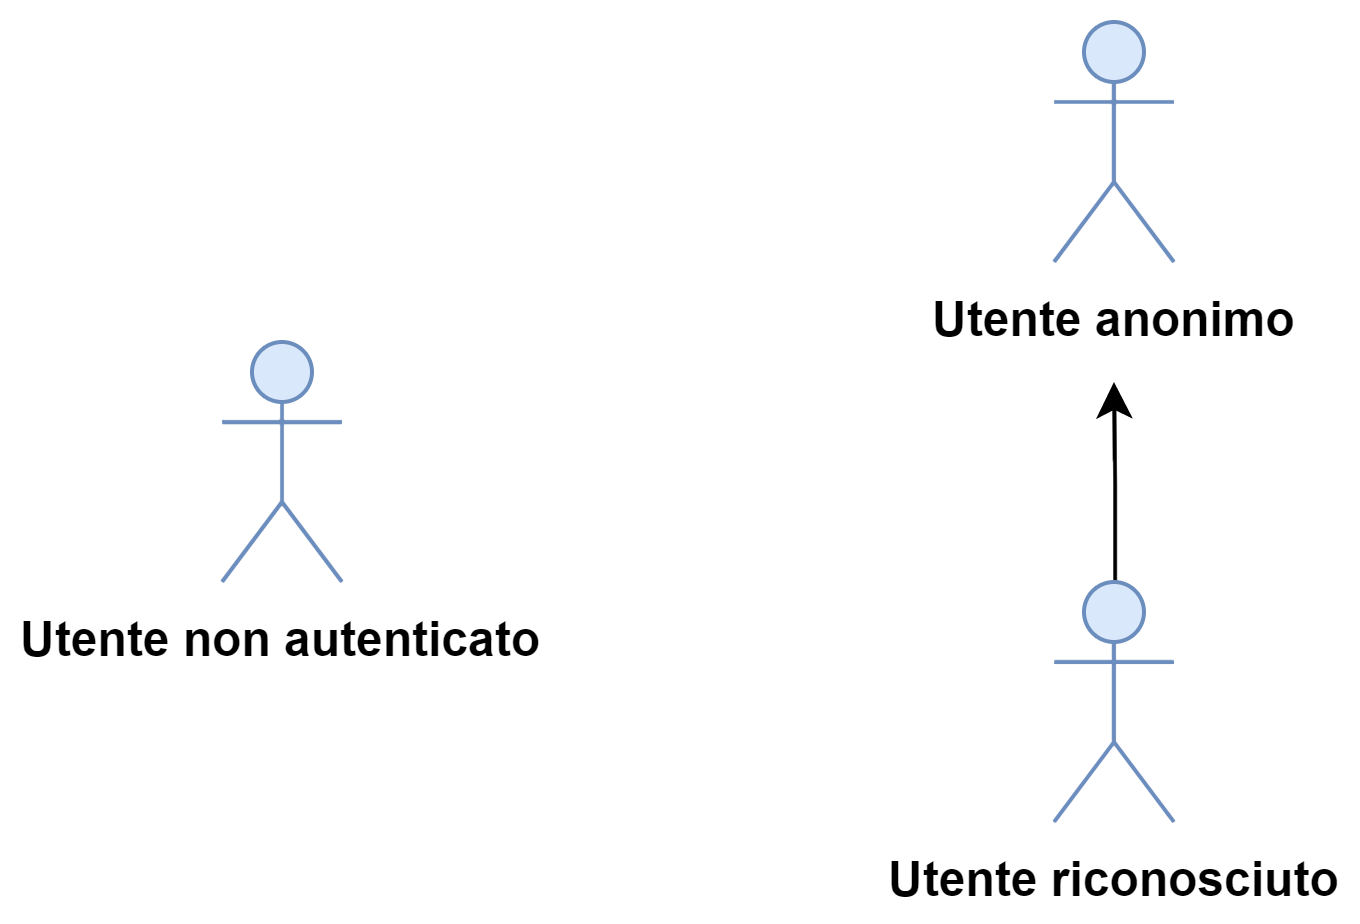
\includegraphics[scale=0.6]{Sezioni/UseCase/Immagini/Utenti.png}
\end{figure}

\paragraph{Utente non autenticato}\mbox{}\\ \\
Utente non ancora autenticato all'applicazione che può avere o non avere le credenziali per autenticarsi.
\paragraph{Utente anonimo}\mbox{}\\ \\
Utente autenticato che può venire tracciato all'interno di una \glo{organizzazione} senza fornire dettagli sulla propria identità.
\paragraph{Utente riconosciuto}\mbox{}\\ \\
Utente autenticato che è attualmente tracciato all'interno di una precisa \glo{organizzazione} fornendo dettagli sulla propria identità.
L'utente si è precedentemente autenticato presso l'\glo{organizzazione} tramite LDAP.



\subsubsection{Attori Amministratori}
\begin{figure}[h]
  \caption{Gerarchia degli amministratori}
  \centering
    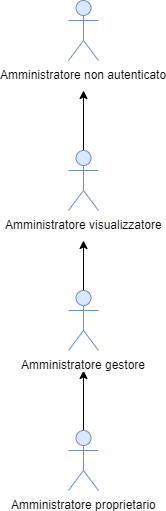
\includegraphics[scale=0.6]{Sezioni/UseCase/Immagini/Amministratori.png}
\end{figure}


\paragraph{Amministratore non autenticato}\mbox{}\\ \\
Amministratore non ancora autenticato nel sistema che ha già le credenziali per autenticarsi.
\paragraph{Amministratore autenticato}\mbox{}\\ \\
Amministratore che si è autenticato nel sistema.
\paragraph{Amministratore proprietario}\mbox{}\\ \\
Amministratore autenticatosi con il ruolo di proprietario dell'\glo{organizzazione}.
Si trova al gradino più alto della gerarchia degli amministratori e dispone delle seguenti funzioni:
\begin{itemize}
\item Gestire l'\glo{organizzazione}, ovvero modificarne i dati (come nome, descrizione, ecc.) e le superfici geografiche per il \glo{tracciamento} degli utenti
\item Gestire gli amministratori, cioè la loro nomina, rimozione e modifica dei privilegi
\item Monitorare gli accessi
\item Eliminare l'\glo{organizzazione}
\end{itemize}
Il proprietario dell'\glo{organizzazione} può nominare altri amministratori.
\paragraph{Amministratore gestore}\mbox{}\\ \\
Amministratore autenticatosi con il ruolo di gestore. 
Si trova al secondo gradino della gerarchia degli amministratori e dispone delle seguenti funzioni:
\begin{itemize}
\item Gestire l'\glo{organizzazione}
\item Monitorare gli accessi
\end{itemize}
\paragraph{Amministratore visualizzatore}\mbox{}\\ \\
Amministratore autenticatosi con il ruolo di visualizzatore.
Escludendo l'amministratore non autenticato si trova all'ultimo gradino della gerarchia degli amministratori e può compiere solo la seguente funzione:
\begin{itemize}
\item Monitorare gli accessi
\end{itemize}

%Alternativa in caso esista una gerarchia a 3 livelli



